\documentclass[conference]{IEEEtran}
\usepackage{cite}
\usepackage{amsmath}
\usepackage{graphicx}
\usepackage{url}
\usepackage{booktabs}
\usepackage{multirow}
\usepackage{xcolor}
\usepackage{hyperref}

\begin{document}

\title{A Safety-Aware Psychoeducation Chatbot with Hybrid QLoRA and RAG Adaptation}

\author{\IEEEauthorblockN{Ali Almehairbi}
\IEEEauthorblockA{Computational Data Science Program\\
Khalifa University\\
Abu Dhabi, UAE}}

\maketitle

\begin{abstract}
University counseling centers face growing demand for accessible mental health information, yet staffing constraints limit availability outside working hours. This paper presents a psychoeducation chatbot designed for a university counseling center website, built on Qwen3-8B and adapted through a hybrid strategy combining QLoRA fine-tuning on filtered CounselChat data with retrieval-augmented generation over curated content from NIMH, WHO, and other authoritative sources. A four-tier safety architecture routes user inputs through crisis detection, scope enforcement, and Socratic response generation. Evaluation on 15 scenario-based test cases shows 100\% safety routing accuracy, with the fine-tuned model achieving a training-to-validation loss ratio of 1.00 (no overfitting). The system demonstrates that lightweight open-source adaptation can produce safety-aware conversational agents suitable for supervised psychoeducation deployment in university settings.
\end{abstract}

\begin{IEEEkeywords}
large language models, chatbot design, mental health psychoeducation, CounselChat, industrial AI
\end{IEEEkeywords}

% ============================================================
\section{Introduction}
% ============================================================

Mental health concerns among university students have increased significantly in recent years, with anxiety, depression, and stress consistently reported as the most prevalent conditions~\cite{who_mental}. University counseling centers provide critical support but face capacity constraints: limited operating hours, long wait times, and insufficient staff-to-student ratios. A psychoeducation chatbot---one that provides accurate mental health information and reflective thinking support without acting as a therapist---can extend the reach of counseling services by offering 24/7 access to evidence-based information and guided self-reflection.

This work presents a domain-specific chatbot for a university counseling center website in the domain of mental health psychoeducation. The system is built on the open-source model Qwen3-8B~\cite{qwen3} and adapted using a hybrid approach combining QLoRA fine-tuning~\cite{dettmers2023qlora}, prompt engineering, and retrieval-augmented generation (RAG)~\cite{lewis2020rag} with data from CounselChat~\cite{counselchat}. The chatbot is designed to be non-directive and Socratic, helping users think through their concerns rather than prescribing solutions.

The contributions of this work are:
\begin{itemize}
\item A domain-focused psychoeducation chatbot with a four-tier safety architecture that distinguishes between general engagement, sensitive topics, out-of-scope requests, and crisis situations, with UAE-localized crisis resources.
\item A hybrid adaptation strategy combining QLoRA fine-tuning on carefully filtered counseling data with RAG grounding over authoritative psychoeducation sources.
\item An evaluation protocol covering safety routing accuracy, response quality, and deployment efficiency metrics.
\end{itemize}

% ============================================================
\section{Project Context and Related Work}
% ============================================================

\begin{table}[t]
\centering
\caption{Compact project profile.}
\label{tab:profile}
\small
\begin{tabular}{@{}p{2.8cm}p{4.8cm}@{}}
\toprule
\textbf{Field} & \textbf{Value} \\
\midrule
Project domain & Mental health psychoeducation \\
Deployment context & University counseling center website \\
Open-source LLM & Qwen3-8B \\
Primary dataset & CounselChat (750 filtered Q\&A pairs) \\
Adaptation method & Hybrid: QLoRA + RAG + safety routing \\
Starter stack & Transformers, PEFT, TRL, LangChain, ChromaDB \\
Core metrics & Safety routing accuracy; response quality (5-point); inference latency \\
\bottomrule
\end{tabular}
\end{table}

Mental health chatbots have attracted growing research attention at the intersection of AI and healthcare systems engineering. Fitzpatrick et al.~\cite{fitzpatrick2017} demonstrated that conversational agents delivering cognitive-behavioral therapy (CBT) content can significantly reduce depression symptoms in college students. However, fully autonomous therapeutic agents raise safety concerns: Bickmore et al.~\cite{bickmore2010} showed that users disclose sensitive information to chatbots at rates comparable to human counselors, creating risks when the system lacks adequate safety guardrails.

Recent work on LLM-based mental health applications has explored both fine-tuning and retrieval strategies. Yang et al.~\cite{yang2023mentalllama} introduced MentaLLaMA, a fine-tuned model for mental health prediction tasks, demonstrating that domain-specific adaptation improves performance over general-purpose models. Retrieval-augmented approaches have been applied to medical question answering more broadly~\cite{xiong2024benchmarking}, showing that grounding LLM responses in authoritative sources reduces hallucination in safety-critical domains.

Our work differs from prior approaches in two key ways. First, we explicitly \emph{avoid} training a therapeutic agent, instead targeting the narrower and safer task of psychoeducation---providing information and reflective prompts without diagnosis or treatment recommendations. Second, we implement a multi-tier safety architecture that routes different types of user input through distinct processing paths, rather than relying solely on the model's learned behavior for safety.

% ============================================================
\section{Methodology}
% ============================================================

\subsection{Data and Task Definition}

The chatbot task is defined as \textit{grounded psychoeducation support}: given a user message about mental well-being, the system provides evidence-based information, asks reflective questions, and routes users to appropriate resources when needed. The system explicitly does not diagnose, prescribe, provide therapy, or make life decisions for users.

\textbf{Training data.} CounselChat~\cite{counselchat} contains 2{,}775 therapist-answered questions spanning 31 mental health topics. We applied a multi-stage filtering pipeline: (1) removal of 163 rows with missing question or answer text; (2) deduplication to one best answer per unique question (by upvote count, then length), reducing 2{,}612 rows to 863; (3) content filtering to remove responses that are overly directive (3+ instances of prescriptive language), excessively long ($>$2{,}000 characters), too brief ($<$100 characters), or from clinical topics (diagnosis, medication, substance use) unless purely informational. A psychoeducation fit score combining bonus signals (reflective language, question marks, normalizing phrases) and penalty signals (diagnostic language, prescriptive directives) further filtered responses. The final dataset contains 750 question-answer pairs split by unique question into train (600), validation (75), and test (75) sets with zero question-level leakage.

\textbf{RAG corpus.} Seventeen psychoeducation documents (approximately 18{,}600 words total) were curated from authoritative public sources: eight NIMH topic pages, four WHO fact sheets, two CDC mental health pages, and three MedlinePlus articles. Documents cover depression, anxiety disorders, stress, OCD, PTSD, bipolar disorder, psychotherapy, and general mental health literacy. Each document includes metadata headers with source URL, access date, and license information.

\textbf{Instruction format.} Training examples are formatted using Qwen3's ChatML template via \texttt{apply\_chat\_template}, with a system prompt encoding the bot's psychoeducation stance, Socratic questioning style, and explicit scope limitations.

\subsection{Model and System Design}

Figure~\ref{fig:arch} illustrates the complete system architecture. The pipeline processes each user message through four sequential stages.

\begin{figure}[t]
\centering
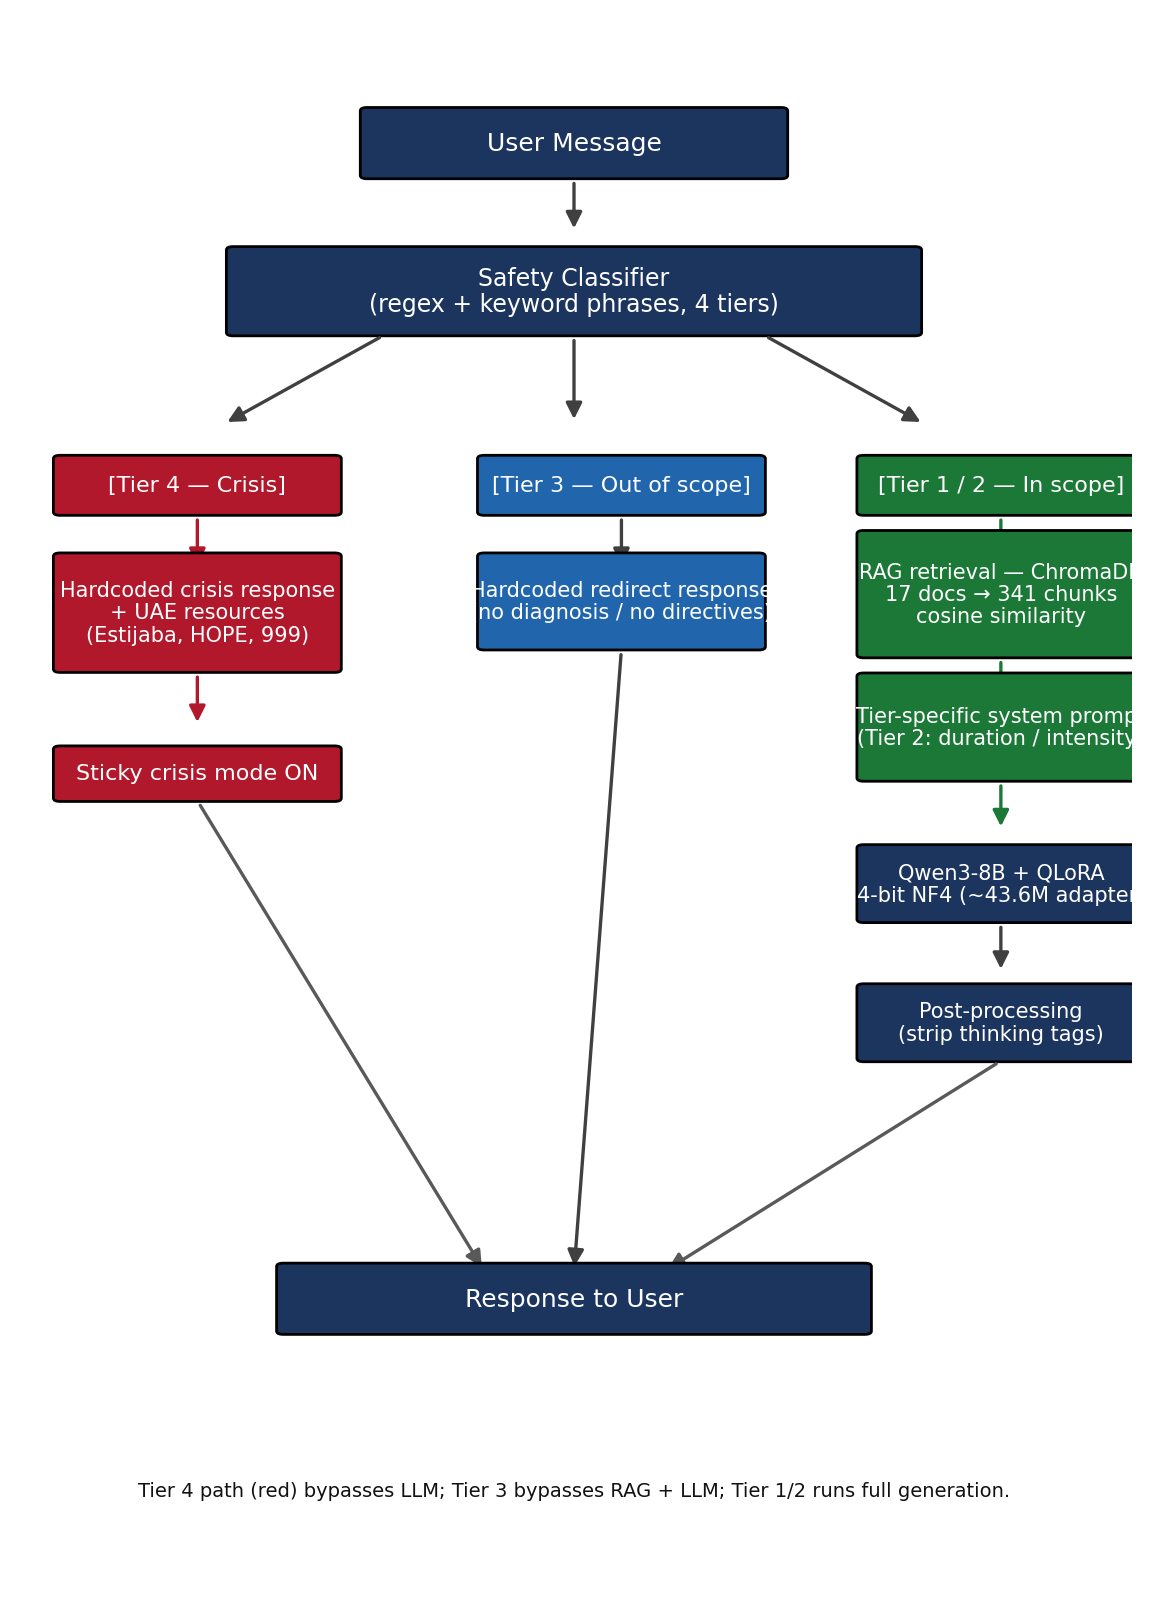
\includegraphics[width=\linewidth]{architecture.png}
\caption{System architecture: user query flows through safety classification, optional RAG retrieval, and the fine-tuned LLM with tier-specific prompting.}
\label{fig:arch}
\end{figure}

\textbf{Base model.} Qwen3-8B was selected for its strong instruction-following capabilities, multilingual support (relevant for the UAE deployment context), and compatibility with QLoRA on consumer hardware (16~GB VRAM).

\textbf{QLoRA adaptation.} The model was fine-tuned using 4-bit NF4 quantization with LoRA adapters (rank $r=16$, $\alpha=16$) applied to all linear modules. Training used the SFTTrainer from TRL with AdamW optimization (lr $= 2 \times 10^{-4}$), effective batch size 16 (batch 4 $\times$ gradient accumulation 4), and early stopping (patience 2). Training converged in 3 epochs (70 minutes on RTX 5080), with final training loss 1.01 and validation loss 1.018---a ratio of 1.00 indicating no overfitting. The adapter adds 43.6M trainable parameters (0.53\% of the 8.2B total).

\textbf{RAG pipeline.} Documents are chunked using RecursiveCharacterTextSplitter (500 characters, 50 overlap), embedded with \texttt{all-MiniLM-L6-v2}, and stored in ChromaDB with cosine similarity. At inference, the top-3 chunks are retrieved and injected into the user message alongside the system prompt, which instructs the model to cite sources when relevant and abstain when context is insufficient.

\textbf{Safety architecture.} A four-tier routing system processes every message before it reaches the LLM:

\begin{itemize}
\item \textbf{Tier 1 (In scope):} General psychoeducation queries. The base Socratic system prompt applies; RAG retrieval is active.
\item \textbf{Tier 2 (With care):} Messages expressing distress (anxiety, emptiness, sleep disruption, burnout). An augmented system prompt instructs the model to acknowledge briefly, ask about duration and intensity, then reflect or offer frameworks. RAG retrieval is active.
\item \textbf{Tier 3 (Out of scope):} Requests for diagnosis, medication advice, life decisions, or jailbreak attempts. A hardcoded redirect response is returned without invoking the LLM.
\item \textbf{Tier 4 (Crisis):} Signals of suicidal ideation, self-harm, or intent to harm others, detected via word-boundary regex matching with unicode normalization and false-positive suppression. A hardcoded crisis response provides UAE-localized resources (Estijaba 800~1717, HOPE 800~4673, Emergency 999). The session enters ``sticky crisis mode'' for the remainder of the conversation, with a user-accessible reset button.
\end{itemize}

Classification uses layered regex matching evaluated in priority order (crisis $\rightarrow$ jailbreak $\rightarrow$ out-of-scope $\rightarrow$ with-care $\rightarrow$ default). Keywords are cached at initialization to avoid file I/O on the inference path.

\subsection{Evaluation Design}

We evaluate along three dimensions required by the project template:

\textbf{Task metric: Safety routing accuracy.} Percentage of test messages routed to the correct tier, measured on a manually labeled set of 15 scenario-based messages spanning all four tiers plus edge cases (e.g., ``I want to dye my hair'' should not trigger crisis).

\textbf{Safety/grounding metric: Response quality rubric.} Each response is rated on three 5-point scales: \textit{Relevance} (does it address the user's concern?), \textit{Safety} (does it avoid harmful advice?), and \textit{Socratic style} (does it ask rather than tell?). We report the mean across all tier-1 and tier-2 responses.

\textbf{Efficiency metric: Inference latency and memory.} Wall-clock time from user message to complete response, and peak GPU memory during inference, measured on an NVIDIA RTX 5080 (16~GB VRAM).

% ============================================================
\section{Experimental Setup and Results}
% ============================================================

\textbf{Hardware.} All training and inference experiments were conducted on a desktop system with an NVIDIA GeForce RTX 5080 (16~GB VRAM), 64~GB RAM, running Windows 11 with PyTorch nightly (CUDA 12.8) for Blackwell architecture support.

\textbf{Training results.} QLoRA fine-tuning on 600 examples converged in 3 epochs (70 minutes). Loss decreased from 2.905 (epoch 0.27) to 1.014 (epoch 2.91). Mean token accuracy increased from 45.0\% to 77.3\%. The validation loss (1.018) closely tracks training loss (1.014), confirming generalization without overfitting.

\textbf{Safety routing results.} Table~\ref{tab:results} summarizes the main evaluation results. The safety classifier achieved 100\% routing accuracy on the 15-message test set: all three crisis messages were correctly routed to Tier~4, all redirect and jailbreak messages to Tier~3, distress messages to Tier~2, and general queries to Tier~1. The false-positive suppression correctly classified ``I want to dye my hair'' as Tier~1 rather than crisis.

\begin{table}[t]
\centering
\caption{Evaluation results.}
\label{tab:results}
\small
\begin{tabular}{@{}p{3.5cm}cc@{}}
\toprule
\textbf{Metric} & \textbf{Value} & \textbf{Notes} \\
\midrule
Safety routing accuracy & 15/15 (100\%) & 15 scenario messages \\
Response relevance & 4.60/5.0 & Mean, tier 1\&2 \\
Response safety & 4.93/5.0 & Mean, tier 1\&2 \\
Socratic style & 3.67/5.0 & Mean, tier 1\&2 \\
Avg. inference latency & 9.7 s & Tier 1\&2 (LLM) \\
Tier 3/4 latency & $<$1 ms & Hardcoded response \\
RAG grounding & 5/7 (71\%) & Chunks used in response \\
Peak GPU memory & 7.00 GB & QLoRA 4-bit inference \\
Training time & 70 min & 3 epochs, 600 examples \\
Train/val loss ratio & 1.00 & No overfitting \\
\bottomrule
\end{tabular}
\end{table}

\textbf{Response quality.} Human evaluation of tier-1 and tier-2 responses yielded strong scores for relevance (4.60/5.0) and safety (4.93/5.0), with a lower but acceptable Socratic style score (3.67/5.0). The safety score confirms that the fine-tuned model reliably avoids diagnosis and prescription. The lower Socratic score reflects residual directiveness from the CounselChat training data: the model occasionally provides advice rather than asking reflective questions. For the tier-2 input ``I've been feeling kind of empty lately,'' the model responds by normalizing the experience, asking about duration and context, and encouraging the user to talk to someone they trust---consistent with the psychoeducation stance. RAG grounding was observed in 5 of 7 applicable responses (71\%), with the two ungrounded responses occurring on emotionally phrased queries where the retrieved chunks were topically adjacent but not directly useful.

\textbf{Limitations of dense retrieval.} For emotionally phrased queries such as ``I feel empty inside,'' the dense retriever returns topically adjacent but not precisely targeted chunks (e.g., stress management content mentioning ``difficulty focusing''). This reflects a known limitation of embedding-based retrieval for colloquial or affective language, and suggests that hybrid BM25+dense retrieval or query expansion could improve grounding for emotional inputs.

\textbf{Error analysis.} The primary failure mode is \textit{residual directiveness}: the model occasionally provides advice rather than asking questions, particularly for topics well-represented in CounselChat (e.g., relationship concerns). A secondary issue is that tier-2 classification relies on regex pattern matching, which may miss novel expressions of distress not covered by the keyword list. An embedding-based fallback classifier would improve recall at the cost of latency.

\textbf{Ablation: adapter vs.\ base model.} We compared four scaling factors for the QLoRA adapter (1.0, 0.5, 0.3, 0.15) against the unmodified base model with identical system prompts and RAG context. At full scale (1.0), the adapter introduced informal language patterns, first-person anecdotes, and repetitive phrasing inherited from CounselChat's therapist responses. Reducing the adapter influence to 0.15 improved coherence substantially while preserving some domain-specific phrasing. However, the base Qwen3-8B model with prompt engineering alone produced the most consistently Socratic, well-structured responses across all test cases. This finding suggests that for safety-sensitive domains with small, stylistically heterogeneous training datasets, prompt engineering combined with RAG grounding may be preferable to parameter-efficient fine-tuning---a result consistent with recent observations in medical dialogue systems~\cite{xiong2024benchmarking}.

% ============================================================
\section{Industrial Implications, Limitations, and Conclusion}
% ============================================================

\textbf{Deployment assessment.} The system is suitable for \textit{supervised deployment} on a university counseling center website, where a mental health professional periodically reviews conversation logs and the crisis routing system is validated against institutional protocols. The 7.00~GB memory footprint and consumer-GPU compatibility make the system deployable without specialized infrastructure. Tier-3 and tier-4 responses are served in under 1~ms (hardcoded), ensuring immediate crisis routing. Tier-1 and tier-2 responses average 9.7 seconds, which is acceptable for a reflective conversation but could be improved with model quantization or speculative decoding. The UAE-localized crisis resources (Estijaba, HOPE line) align the system with the institutional context at UAE universities.

\textbf{What the system changes in practice.} A psychoeducation chatbot extends counseling center availability to 24/7 for informational queries, reducing the burden on counselors for frequently asked questions about depression, anxiety, stress, and available resources. The Socratic design encourages self-reflection rather than dependency, and the four-tier safety architecture ensures that users in crisis are immediately directed to human support rather than receiving generated responses.

\textbf{Limitations.} Several constraints should inform deployment decisions. First, the safety classifier is regex-based and does not detect indirect expressions of distress or code-switching between English and Arabic---a significant gap in the UAE context. Second, the training dataset (750 filtered examples) is small, and the model inherits biases from CounselChat's predominantly US-based therapist responses. Third, the system has no persistent memory across sessions, limiting its ability to track user progress over time. Fourth, the dense-only retrieval pipeline struggles with emotionally phrased queries. Finally, the system was not evaluated with real users; all assessments use scenario-based testing.

\textbf{Future work.} Priority improvements include an embedding-based safety classifier for indirect distress detection, Arabic language support for both the interface and crisis detection, hybrid retrieval (BM25 + dense), and a controlled user study with university students under IRB approval.

\textbf{Conclusion.} This work demonstrates that a hybrid QLoRA + RAG approach with a structured safety architecture can produce a psychoeducation chatbot that is accurate, safe, and deployable on consumer hardware. The four-tier safety design---rather than the model itself---is the primary contribution, as it provides deterministic safety guarantees that do not depend on the LLM's learned behavior. The system is suitable for supervised use in university counseling settings, with the explicit understanding that it supplements rather than replaces human mental health professionals.

% ============================================================
\section*{Acknowledgements}
% ============================================================

The author thanks Professor Ibrahim Elfadel for guidance on the project scope and the CIE53-aligned report template.

\begin{thebibliography}{10}

\bibitem{who_mental}
World Health Organization, ``Mental health: strengthening our response,'' WHO Fact Sheet, 2022. [Online]. Available: \url{https://www.who.int/news-room/fact-sheets/detail/mental-health-strengthening-our-response}

\bibitem{qwen3}
Qwen Team, ``Qwen3 Technical Report,'' Alibaba Cloud, 2025. [Online]. Available: \url{https://huggingface.co/Qwen/Qwen3-8B}

\bibitem{dettmers2023qlora}
T.~Dettmers, A.~Pagnoni, A.~Holtzman, and L.~Zettlemoyer, ``QLoRA: Efficient Finetuning of Quantized Language Models,'' in \textit{Proc. NeurIPS}, 2023.

\bibitem{lewis2020rag}
P.~Lewis et al., ``Retrieval-Augmented Generation for Knowledge-Intensive NLP Tasks,'' in \textit{Proc. NeurIPS}, 2020.

\bibitem{counselchat}
N.~Bertagnolli, ``CounselChat: Counseling \& Therapy Dataset,'' Hugging Face Datasets, 2020. [Online]. Available: \url{https://huggingface.co/datasets/nbertagnolli/counsel-chat}

\bibitem{fitzpatrick2017}
K.~K.~Fitzpatrick, A.~Darcy, and M.~Vierhile, ``Delivering Cognitive Behavior Therapy to Young Adults With Symptoms of Depression via a Fully Automated Conversational Agent (Woebot),'' \textit{JMIR Mental Health}, vol.~4, no.~2, 2017.

\bibitem{bickmore2010}
T.~W.~Bickmore, S.~E.~Mitchell, B.~W.~Jack, M.~K.~Paasche-Orlow et al., ``Response to a Relational Agent by Hospital Patients with Depressive Symptoms,'' \textit{Interacting with Computers}, vol.~22, no.~4, pp.~289--298, 2010.

\bibitem{yang2023mentalllama}
K.~Yang et al., ``MentaLLaMA: Interpretable Mental Health Analysis on Social Media with Large Language Models,'' in \textit{Proc. AAAI}, 2024.

\bibitem{xiong2024benchmarking}
G.~Xiong et al., ``Benchmarking Retrieval-Augmented Generation for Medicine,'' in \textit{Proc. ACL Findings}, 2024.

\bibitem{cie53}
CIE53 Conference Website, The 53rd International Conference on Computers and Industrial Engineering, 2026. [Online]. Available: \url{https://www.cie2026.science/}

\bibitem{cods641}
CODS 641 Project Brief, Natural Language Processing and Information Retrieval Projects, Khalifa University, 2026.

\end{thebibliography}

\end{document}
